\section{Results}
\label{sec:results}
In the next sections, I present the main results of my experiment to support our claim that SafraFT is correct, to show how SafraFT compares to SafraFS and to exemplify the performance of SafraFT under the presence of faults.

The observations are based on runs of the system described in \cref{sec:methods} on the DAS-4 cluster at the Vrije Universiteit of Amsterdam.
I measured runs on networks from 50 to 2000 nodes for SafraFT and SafraFS.
SafraFT was also tested with 1 to 5 nodes failing per run (dubbed 5n) and with 90\% node failure.
\cref{table:runs} presents how many repetitions of each configuration were run.

The raw data including a manual on how to interpret it can be found TODO here.
\begin{table}[]
	\centering
	\begin{tabular}{@{}lllll@{}}
		\toprule
		Algorithm & Network              & Faults & Repetitions  & \#Instances / DAS-4 node   \\ \midrule
		SafraFS   & 50                   & 0      & 100          & 25                    \\
		SafraFS   & 250/500/1000/2000    & 0      & 100          & 125                   \\
		SafraFT   & 50                   & 0      & 100          & 25                    \\
		SafraFT   & 250/500/1000/2000    & 0      & 100          & 125                   \\
		SafraFT   & 50                   & 5n     & 100          & 25                    \\
		SafraFT   &    250/500/1000/2000 & 5n     & 100          & 125                   \\
		SafraFT   & 50                   & 90\%   & 100          & 25                    \\
		SafraFT   &    250/500/1000/2000 & 90\%   & 100          & 125                   \\ \bottomrule
	\end{tabular}
	\caption{List of all configurations run. Per physical DAS-4 node with 8 cores multiple virtual instances in their own processes where run (columm '\#Instances / DAS-4 node`). The amount of physical node equates to network size divided by instances.}
	\label{table:runs}
\end{table}

\subsection{Correctness of SafraFT}
\label{ssec:correctness}
The experiment is aimed to support our paper with a practical, correct application of our algorithm.
Towards this goal, I build multiple correctness checks into the experiment. 

To assure nothing happens after termination detection, the application logs if any messages are received or actions are executed after termination has been detected and announced. 
The analysis tools provided with the experiment point these logs out to make sure they are not overlooked.

To proof termination is not detected too early, I use offline analysis (see \cref{ssec:offline-analysis}) to determine the point of actual termination and verify that detection happened after.
All 1000 runs using SafraFT under the presence of faults confirm that termination was never detected too early.

However, the experiment revealed that the framework for termination chosen to develop SafraFT is not complete and does not cover all cases for my experimental setup.
SafraFT is developed for the following and commonly used definition of termination:
\begin{enumerate}
	\item All nodes are passive
	\item No messages are in the channels
\end{enumerate}
This definition is based on the fact that a node is either an initiator or can only become active if it receives a message. 
Anyhow, in the presence of failures and if additionally, the outcome of the algorithm depends on the set of alive nodes, nodes might get activated by the detection of a failure.
For example, when Chandy Misra builds a sink tree, nodes that detect a crash of their parents will become active afterwards to find a new path towards the root.
This fact leads to the following concrete scenario in which the definition of termination assumes termination too early: let us consider the situation that all nodes are passive and no messages are in the channel. 
In other words, the system terminated by our definition.
Node \co{X} forwards the token to \co{Y} and crashes afterwards. 
Node \co{Y} calls announce after receipt of the token.
Assume node \co{Z} is a child of \co{X} and detects the crash of its parent, it becomes active after termination has been formally reached and announced.
By sending out \co{REQUEST} messages, it might activate other nodes again.

To conclude, the definition of termination that our algorithm is built upon does not fully capture the reality of our basic algorithm which could lead to an early detection of termination.

To verify if situations like this actually occur during the experiment, I analysed the logs generated according to the definition of termination used to develop SafraFT (see above) and the following definition:
\begin{enumerate}
	\item All nodes are passive
	\item No messages are in the channels
	\item Termination is postponed until the last node failure that leads to action is detected
\end{enumerate}
\label{extended-definition}

As stated above, SafraFT did never detect termination too early according to its definition.
According to the extended definition, it detects termination to early in \OutputFileNum{figures/early-termination.txt} out 1500 runs.
However, due to the fact that repairing the sink tree after detecting a parent crash is quite fast and there is a short time window to do so while the announce call propagates to all nodes, only in \OutputFileNum{figures/early-termination-corrupted.txt} of these cases that leads to the situation that basic activity happened after detected termination.


I carefully reviewed each repetition in which termination is detected too early according to the extended definition to verify that early termination detection is in fact caused by a situation as described above.
The logs of these runs provide a summary of all detections of parent crashes close to the announce call to ease this procedure.

\subsection{Comparision of Safra versions}
This section compares SafraFS and SafraFT. 
Additionally, it analysis how the network size influences both algorithms.

The number of tokens sends in total and after termination is presented in \cref{fig:tokens-and-tokens-after}.

\begin{sidewaysfigure}[ht]
	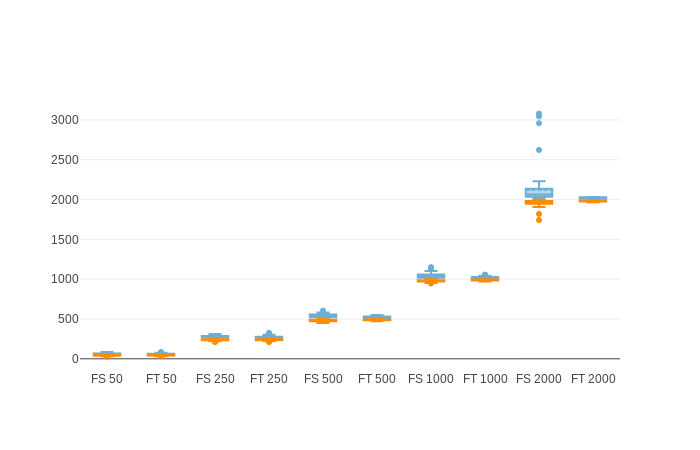
\includegraphics{figures/tokens-and-tokens-after.png}
	\caption{Tokens (blue) and tokens after termination (orange) for SafraFT and SafraFS in fault free runs for all network sizes.}
	\label{fig:tokens-and-tokens-after}
\end{sidewaysfigure}

The key observation is that SafraFS and SafraFT behave highly similar except for networks with 2000 nodes where SafraFS results show much more variance and some extraordinary outliers.
For all other network sizes, the differences are small.
SafraFT sends slightly fewer tokens in average.
Also, the results for SafraFS show a slightly higher variance.
Most likely these differences are caused by implementation details and are not generalizable.

As one would expect, the number of tokens grows linearly with the network size, again with 2000 node networks being an exception (here it grows overlinearly).
Note that the first network size is 5 times smaller than the second for bigger networks the size doubles for each run.

The exceptional results for networks with 2000 nodes might be caused by the fact that Chandy Misra does not scale linearly with the network size. 
This does not directly affect the number of tokens. 
Therefore, it does not show for smaller networks but only with 2000 nodes.

The bit complexity of SafraFS is constant.
In this experiment, each token of SafraFS contains 12 bytes.
SafraFT has a bit complexity linearly to the network size (when no faults occur).
For a network of 50 nodes, each token has 420 bytes; a token in a 2000 node network counts 16020 bytes.
The growth can be described by $bytes = 8 * <network size> + 20$.

I measured two kinds of timing metrics in this experiment.
On the one hand, there are the wall time metrics of total time and total time after termination.
Both were recorded in elapsed seconds between two events. 
For total time, these events are the start of the basic algorithm and the notification to the last node about termination. 
Total time after termination is defined as the number of seconds between the actual termination (extended termination definition from \cref{ssec:correctness}) and the event of a node calling
announce. % TODO is that too much explanation, does everybody but you know so?
On the other hand, there are basic, Safra and Safra after termination processing times (including the time needed to send messages).
These are the accumulated times all instances needed to process basic or Safra functions.
Total times and processing times are measured in a different way and should not be compared directly for multiple reasons. 
First, while total times include idle times, time spent for logging, processing time do not include these.
Secondly, total time is wall time between two events and processing times are accumulated over all processes. 
One particular example of when this leads to differences is that time spent concurrently by two processes counts double in processing time metrics but only once in wall time metrics.

\begin{table}
	\centering
	\begin{tabular}{rrrrrr||rr}%
		\toprule
		\multicolumn{1}{c}{Network} &
		\multicolumn{1}{c}{Basic} &
		\multicolumn{1}{c}{Safra FS} &
		\multicolumn{1}{c}{Safra FT} &
		\multicolumn{1}{c}{Overhead FS} &
		\multicolumn{1}{c||}{Overhead FT} &
		\multicolumn{1}{c}{Safra FS}   &
		\multicolumn{1}{c}{Safra FT} 
		\\
		\midrule
		\csvreader[head to column names]{figures/processing-times.csv}{}
		{\\\networkSize & \basic & \FS & \FT  & \FSoverhead \% & \FToverhead \% & \FSAfter & \FTAfter}
		\\\bottomrule
	\end{tabular}
	\caption{Total processing times (left) and processing times after termination (right) in seconds and overhead over basic algorithm caused by Safa in percent}
	\label{table:processing-times}
\end{table}

One can observe in \cref{table:processing-times} that SafraFT uses more processing time than SafraFS and much of the additional time is spent between actual termination and termination detection.
Furthermore, one sees that SafraFS times grow roughly linear with the network size while SafraFT timings show a nearly three-fold increase for each network size.
This hints for a change in time complexity between the two versions.

A small sub-experiment of excluding the time spent to send messages from the processing time revealed that most of this difference can be tributed to writing tokens onto the wire.
As we know from a previous paragraph, the number of token send does not differ between the algorithms.
Therefore, I believe that these differences are caused by the higher bit complexity of SafraFT. 
This would explain the total increase in the timing from SafraFS to SafraFT, as well as, the change of time complexity.
The time complexity would change because the increase in network size leads to more token being sent (as in SafraFS) but also to bigger tokens being sent.

The processing time \cref{table:processing-times} also presents a comparison of the time spent on the basic algorithm and both Safra versions.
Although SafraFT uses significantly more time, the overhead on the processing time stays moderate with a maximum of 4.26\% for networks with 50 nodes.
% number
\\
\begin{table}
	\centering
	\begin{tabular}{rrrr||rrr}%
		\toprule
		\multicolumn{1}{c}{Network} &
		\multicolumn{1}{c}{Safra FS} &
		\multicolumn{1}{c}{Safra FT} &
		\multicolumn{1}{c||}{$\Delta$} &
		\multicolumn{1}{c}{SafraFS}  &
		\multicolumn{1}{c}{SafraFT}  &
		\multicolumn{1}{c}{$\Delta$}  \\
		\midrule
		\csvreader[head to column names]{figures/total-times.csv}{}
		{\\\networkSize & \FS & \FT & \difference & \FSAfter & \FTAfter & \differenceAfter}
		\\\bottomrule
	\end{tabular}
	\caption{Wall times total (left) and after termination (right) for SafraFT and SafraFS in seconds with ratios}
	\label{table:total-times}
\end{table}

The same pattern of SafraFT using more time and reacting stronger to an increase in network size is visible for total times in \cref{table:total-times}.
Networks with 250 nodes show an exceptionally high ratio of \OutputFileNum{figures/total-time-ratio-250.txt} between SafraFS and SafraFT.

For SafraFS roughly half of the time is spent after termination for small networks.
In big networks, the part of the time spent after termination is lower because the fraction spent by the basic algorithm becomes dominant. 

The systems using SafraFT spent the majority of their time to detect termination because of the already noted higher time complexity of SafraFT.

I would like to note that the low processing time overhead of Safra is not in contradiction to a large amount of wall time spent after termination.
These seemingly opposing results arise from the difference between wall time and processing time: the basic algorithm is much more active at the beginning that is when it accumulates a lot of processing time; while Safra causes a lot of idle time in the end when all processes wait for their predecessor to pass on the token. 
This idle time is not included in processing time but wall time does include it.

To conclude, the experiments confirm that the message complexity of SafraFT remains as for the fault sensitive version but its higher bit complexity causes a higher time complexity which leads to a later termination detection. 
Still, SafraFT causes only a moderate processing time overheads between \OutputFileNum{figures/min-ft-processing-time-overhead.txt}\% and \OutputFileNum{figures/max-ft-processing-time-overhead.txt}\%.

\subsection{Influence of faults}
In the following paragraphs, I present and explain the data generated by runs in the presence of node crashes.
I run two highly different scenarios: one considering networks with 1 to 5 nodes failing and one with 90\% of all nodes crashing.
These scenarios are chosen to show SafraFT in both the realistic case of a low number of faults to handle, as well as, an extreme case; with the aim to confirm that SafraFT handles both cases correctly and without unreasonable deterioration in any metric.

I used the extended definition of termination to determine the point of time of actual termination to generate the metrics shown in this section.

\subsubsection{Tokens}
\label{ssec:tokens-faulty}
For both the networks where between 1 and 5 nodes failed, as well as, for the highly faulty runs with 90\% node failure, the number of tokens increased compared to runs without any faults.
Runs with 90\% failure produced even more tokens than runs with only 1 to 5 node failing - except in networks of 2000 nodes where 5n exhibits a higher token sent average.
The data is presented \cref{fig:tokens-and-tokens-after-faulty} and \cref{table:tokens-faulty}.

\begin{sidewaysfigure}[ht]
	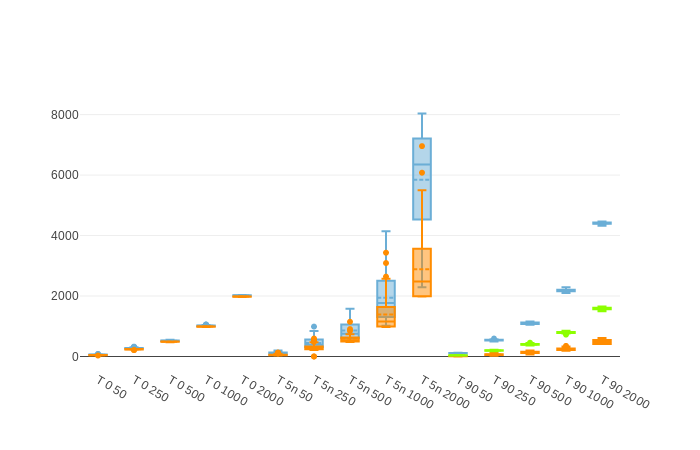
\includegraphics{figures/tokens-and-tokens-after-faulty.png}
	\caption{Tokens (blue) and tokens after termination (orange) for SafraFT on the x-axis for 5 network sizes and 5n and 90\% fault configurations on the y-axis.        Backup tokens in green, shown only for 90\%}
	\label{fig:tokens-and-tokens-after-faulty}
\end{sidewaysfigure}
% TODO outliers to thick
\begin{table}
	\centering
	\begin{tabular}{rrrrrr||rrrrr}%
		\toprule
		\multicolumn{1}{c}{Network} &
		\multicolumn{1}{c}{No faults} &
		\multicolumn{1}{c}{5n} &
		\multicolumn{1}{c}{$\Delta$} &
		\multicolumn{1}{c}{90\%} &
		\multicolumn{1}{c||}{$\Delta$} &
		\multicolumn{1}{c}{No faults} &
		\multicolumn{1}{c}{5n} &
		\multicolumn{1}{c}{$\Delta$} &
		\multicolumn{1}{c}{90\%} &
		\multicolumn{1}{c}{$\Delta$} \\
		\midrule
		\csvreader[head to column names]{figures/tokens-faulty.csv}{}
		{\\\networkSize & \noFaults & \fiveN & \differenceFiveN & \ninety & \differenceNinety &
			\noFaultsAfter & \fiveNAfter & \differenceFiveNAfter & \ninetyAfter & \differenceNinetyAfter }
		\\\bottomrule
	\end{tabular}
	\caption{Tokens in total (left) and after termination (right) for different fault scenarios compared to fault-free networks.}
	\label{table:tokens-faulty}
\end{table}

Otherwise, the two types of fault simulation had a highly different influence on the tokens and tokens after termination metrics.

Between 1 and 5 node failures lead to a strong increase in the variance of tokens sent and in tokens sent after termination.
This seems reasonable because runs with failing nodes might lead to more different situations as runs without fails e.g. one failing node could easily cause an extra token round when it leads to a backup token being issued and forwarded (this token is marked black until it reaches the node it originates from), at the same time, a single failing node that is a leaf in a Chandy Misra sink tree and that crashes just before the call of announce at the successor  causes no further activity.
The same example provides an idea of why the variability increases in big networks. 
That is because one extra round in a big network has a much higher impact on the token count than in a small network.

The phenomenon explained in the last paragraph most likely causes the extremely high maximum of tokens sent and over linear increase of the average number of tokens in networks with 2000 nodes for 1 to 5 nodes failing.

Other than networks with one to 5 failing nodes, networks with up to 90\% node failure lead to a similar low variance in tokens and tokens after termination as fault-free networks.
A likely explanation is that the low survival rate of 1 out of 10 instances leads to less different scenarios than in the fault scenario treated in the last paragraphs.

Even though only one 10th of the nodes survive to participate in the latter token rounds, the highly faulty networks produced more tokens than any other network of the same size.
That is most likely due to the high amount of backup tokens generated (also shown in \cref{fig:tokens-and-tokens-after-faulty})
As mentioned above there is one exception: networks with 2000 cause more token to be generated in 5n networks than in networks with 90\% node failure.

Different from all other networks, highly faulty networks exhibit a much lower token to token after termination ratio caused by the low number of nodes alive in the last rounds.

The network size has no clear influence on the overhead in the number of tokens send before or after termination for the 5n scenario up to networks with 500 nodes. 
For bigger networks, more nodes lead to higher overheads.

The size of networks with 90\% node failures is positively correlated to the overhead of tokens in total and has no influence on the overhead of tokens after termination.

\subsubsection{Backup tokens}
The average amount of backup tokens sent for either fault simulation or network size is lower than the number of faults.
This is due to the fact that SafraFT only issues backup tokens when the fault of its successor is detected via the fault detector but not if this fault is noticed by receiving a token.
There are even runs where 1 to 5 nodes fail but no backup token is issued up to networks containing 2000 nodes. 

The other extreme were more backup tokens are issued than faults occur exists as well.
This can be explained by my decision to have node failing after issuing a backup token.
For example, nodes \co{A}, \co{B} and \co{C} follow each other in the ring, node \co{C} fails which is detected by \co{B} and a backup token is issued.
After, issueing the backup token \co{B} fails on detection \co{A} issues a backup token towards \co{C}.
Only then \co{A} detects the failing of \co{C} and issues a second backup token to its new successor.  


\subsubsection{Token size}
\begin{table}
	\centering
	\begin{tabular}{rrrrrr}%
		\toprule
		\multicolumn{1}{c}{Network} &
		\multicolumn{1}{c}{No faults} &
		\multicolumn{1}{c}{5n} &
		\multicolumn{1}{c}{$\Delta$} &
		\multicolumn{1}{c}{90\%} &
		\multicolumn{1}{c}{$\Delta$}  \\
		\midrule
		\csvreader[head to column names]{figures/token-sizes-faulty.csv}{}
		{\\\networkSize & \noFaults & \fiveN & \differenceFiveN & \ninety & \differenceNinety }
		\\\bottomrule
	\end{tabular}
	\caption{Token size averages in bytes for both fault scenarios compared to token size with zero faults.}
	\label{table:token-sizes-faulty}
\end{table}

The average token size increases with faults because the IDs of faulty nodes are propagated by the token (see \cref{table:token-sizes-faulty}).

The influence on token size is constant 8 bytes for networks with 1 to 5 failing nodes.

90\% node failure leads to a linear increase of token bytes to the network size of a factor 1.15.


\subsubsection{Processing Time}
The observations of this chapter are backed by \cref{table:processing-times-faulty}.

As for tokens, one can see an increase in processing times before termination under the presence of faults compared to fault-free runs. Which is no surprise because more tokens were sent.

For runs with 1 to 5 failing node, a higher variability in the processing times before and after termination becomes apparent (not shown in the tables of the report). 
Most likely this is because of the higher diversity of scenarios possible if some nodes fail as explained in \cref{ssec:tokens-faulty}.
As the processing time grows for this runs, so does the processing time after termination.

For highly faulty networks one observes results in line with the results for tokens in these networks.
The variability for processing time before or after termination is not raised compared to fault-free networks.
The processing time taken is even higher than the one for less faulty networks.
Less processing time after termination is spent than for fault-free networks because fewer tokens need to be sent.

An interesting observation is that the difference between fault free processing time to processing time with faults does not necessarily increase with the network size:
with 90\% node failure the differences sink.

% TODO why is this interesting
\begin{table}
	\centering
	\begin{tabular}{rrrrrr||rrrrr}%
		\toprule
		\multicolumn{1}{c}{Network} &
		\multicolumn{1}{c}{No faults} &
		\multicolumn{1}{c}{5n} &
		\multicolumn{1}{c}{$\Delta$} &
		\multicolumn{1}{c}{90\%} &
		\multicolumn{1}{c||}{$\Delta$} &
		\multicolumn{1}{c}{No faults} &
		\multicolumn{1}{c}{5n} &
		\multicolumn{1}{c}{$\Delta$} &
		\multicolumn{1}{c}{90\%} &
		\multicolumn{1}{c}{$\Delta$} \\
		\midrule
		\csvreader[head to column names]{figures/processing-times-faulty.csv}{}
		{\\\networkSize & \noFaults & \fiveN & \differenceFiveN & \ninety & \differenceNinety &
			\noFaultsAfter & \fiveNAfter & \differenceFiveNAfter & \ninetyAfter & \differenceNinetyAfter }
		\\\bottomrule
	\end{tabular}
	\caption{Total processing times (left) and after termination (right) in seconds for different fault scenarios compared to fault-free networks.}
	\label{table:processing-times-faulty}
\end{table}

\subsubsection{Total time}
Total time in faulty networks is presented in  \cref{table:total-times-faulty}.
In line with the observations from the processing time section, one observes:
\begin{itemize}
	\item an increase in total time spent for fault scenarios
	\item a higher variability for time spent before and after termination for less faulty networks
	\item less time spent after termination by highly faulty networks
\end{itemize}

For a network with 90\% node failure, the overhead for total time decreases for network sizes between 50 and 1000 nodes and increases to its maximum for 2000 nodes.
The overhead of time after termination sinks with higher network sizes.
\begin{table}
	\centering
	\begin{tabular}{rrrrrr||rrrrr}%
		\toprule
		\multicolumn{1}{c}{Network} &
		\multicolumn{1}{c}{No faults} &
		\multicolumn{1}{c}{5n} &
		\multicolumn{1}{c}{$\Delta$} &
		\multicolumn{1}{c}{90\%} &
		\multicolumn{1}{c||}{$\Delta$} &
		\multicolumn{1}{c}{No faults} &
		\multicolumn{1}{c}{5n} &
		\multicolumn{1}{c}{$\Delta$} &
		\multicolumn{1}{c}{90\%} &
		\multicolumn{1}{c}{$\Delta$} \\
		\midrule
		\csvreader[head to column names]{figures/total-times-faulty.csv}{}
		{\\\networkSize & \noFaults & \fiveN & \differenceFiveN & \ninety & \differenceNinety &
			\noFaultsAfter & \fiveNAfter & \differenceFiveNAfter & \ninetyAfter & \differenceNinetyAfter }
		\\\bottomrule
	\end{tabular}
	\caption{Total times (left) and after termination (right) in seconds. For different fault scenarios compared to fault-free networks.}
	\label{table:total-times-faulty}
\end{table}



